\section{Virtual Memory Management}
\subsection*{Page Fault}
HW virtual address translation: transparent if succeeds (frame in RAM, no protection violation) (common case), page fault exception if fails.\\
Page fault cases: page not present (valid bit off, OS handles, recursion if dealing with fault in page tables), protection error (OS generates software exception - SIGSEGV (seg fault) or SIGBUS), page not used (valid bit off, could be an auto expanding segment like stack).\\
Reset page table may need update multi-level tables.

\subsection*{Page Placement Policy: any frame}
\subsection*{Page Fetch Policy}
\emph{Demand paging:} only faulting page is fetched. \emph{Prepaging:} other pages can be fetched on page fault. Can also be loaded when starting process.

\subsection*{Page Replacement Algorithms}
Incoming page can be from swap or executable file. If page to be replaced is dirty, need to write back to swap; if clean, can be discarded. Good algorithm have very few page faults: $T_{access}=(1-p)T_{mem}+pT_{page\_fault}$.\\
\emph{Optimal Page Replacement (OPT):} Replace page that will not be used again for the longest time, guarantees min page faults.\
\emph{FIFO:} Evict oldest memory page. (+) simple implementation (OS maintains queue of resident page no.) (-) Belady's Anomaly (more frames, more page faults, since doesn't exploit temporal locality).\\
\emph{Least Recently used (LRU):} Replace page that has not been used in longest time (temporal locality). (-) Hard to implement. Appr. 1: counter, PTE with time-of-use field(forever increasing may overflow), need to search through all pages. Appr. 2: stack of page no. If X referenced, remove from stack and push on top. Replace page at stack bottom.\\
\emph{Second-Chance (CLOCK):}\\
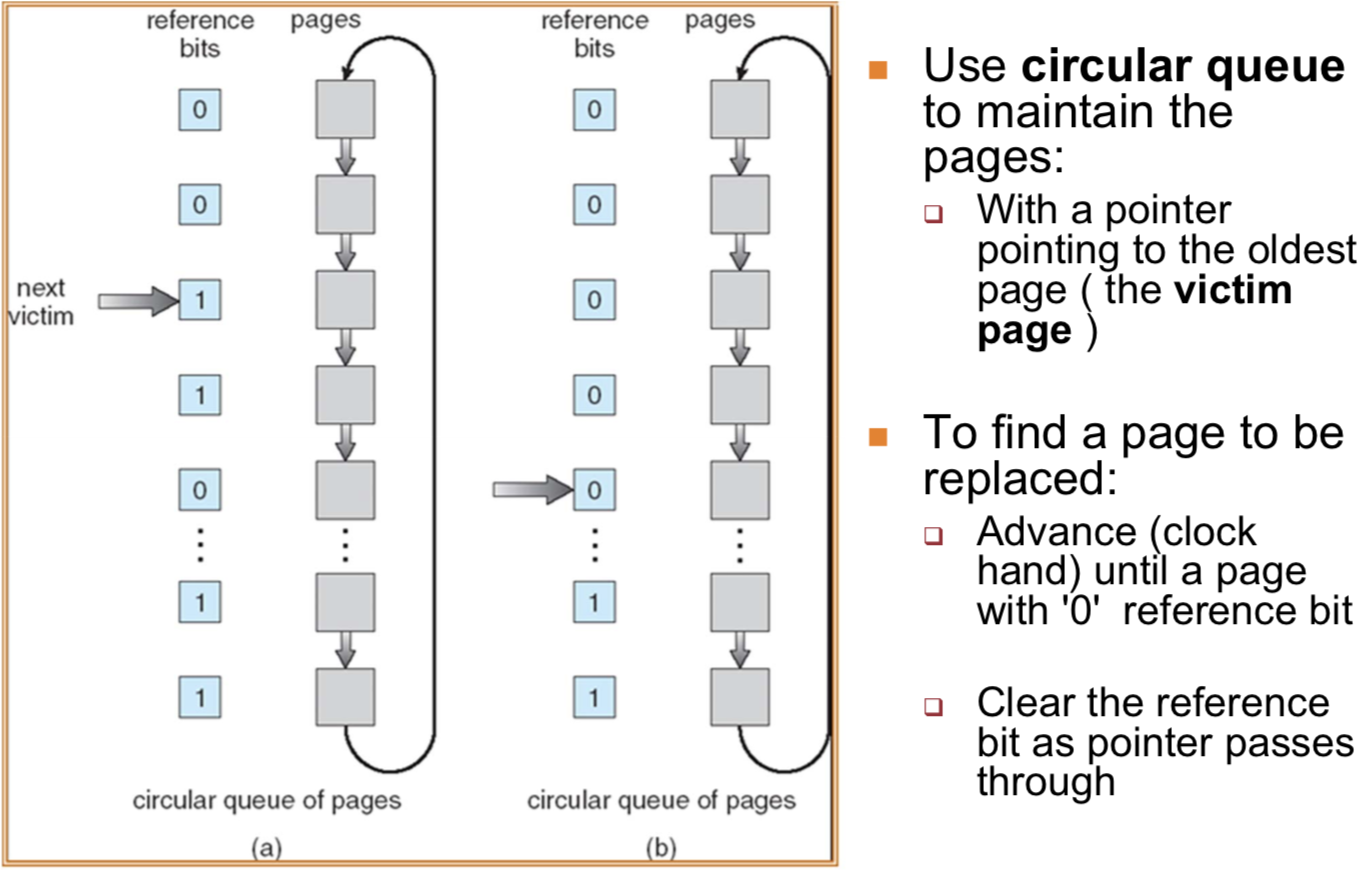
\includegraphics[width=0.8\linewidth]{images/second-chance-page-replacement}\\
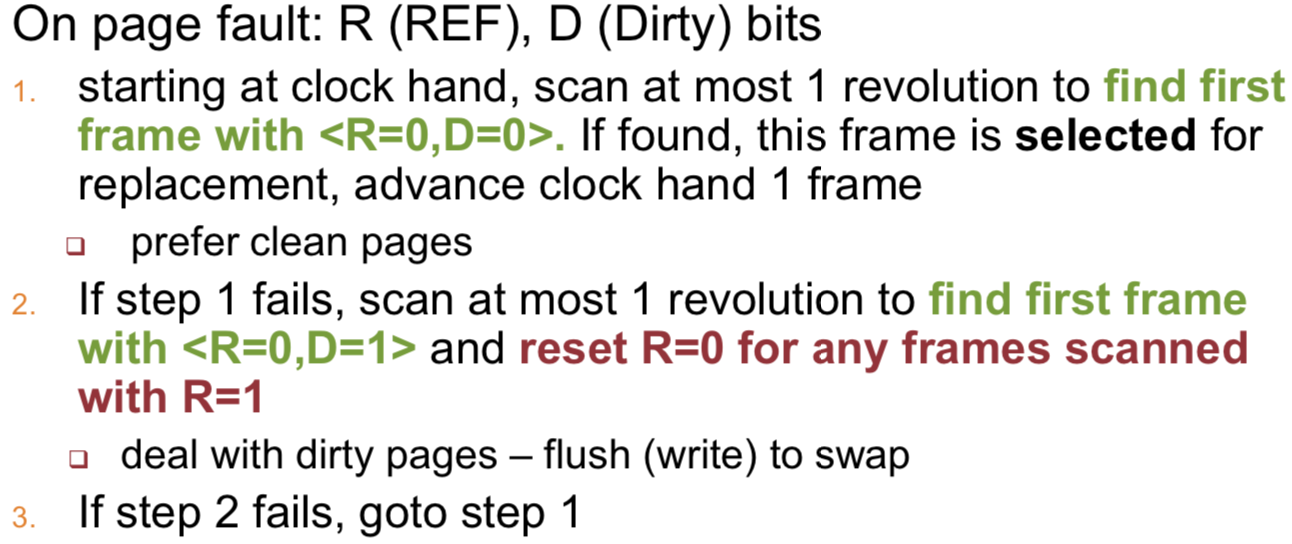
\includegraphics[width=0.9\linewidth]{images/clock_algo}

\subsection*{Frame Allocation}
Equal allocation(N/M), Proportional allocation($size_p/size_{total}*N)$.\\
Local replacement: (+) Stable performance between multiple runs, (-) not enough frame hinder progress. Global replacement: (+) self-adjustment between processes, (-) bad process affects others.\emph{Thrashing:} not enough frame, global -> cascading thrashing, local -> single process hogs I/O.\\
\emph{Working Set Model:}\\
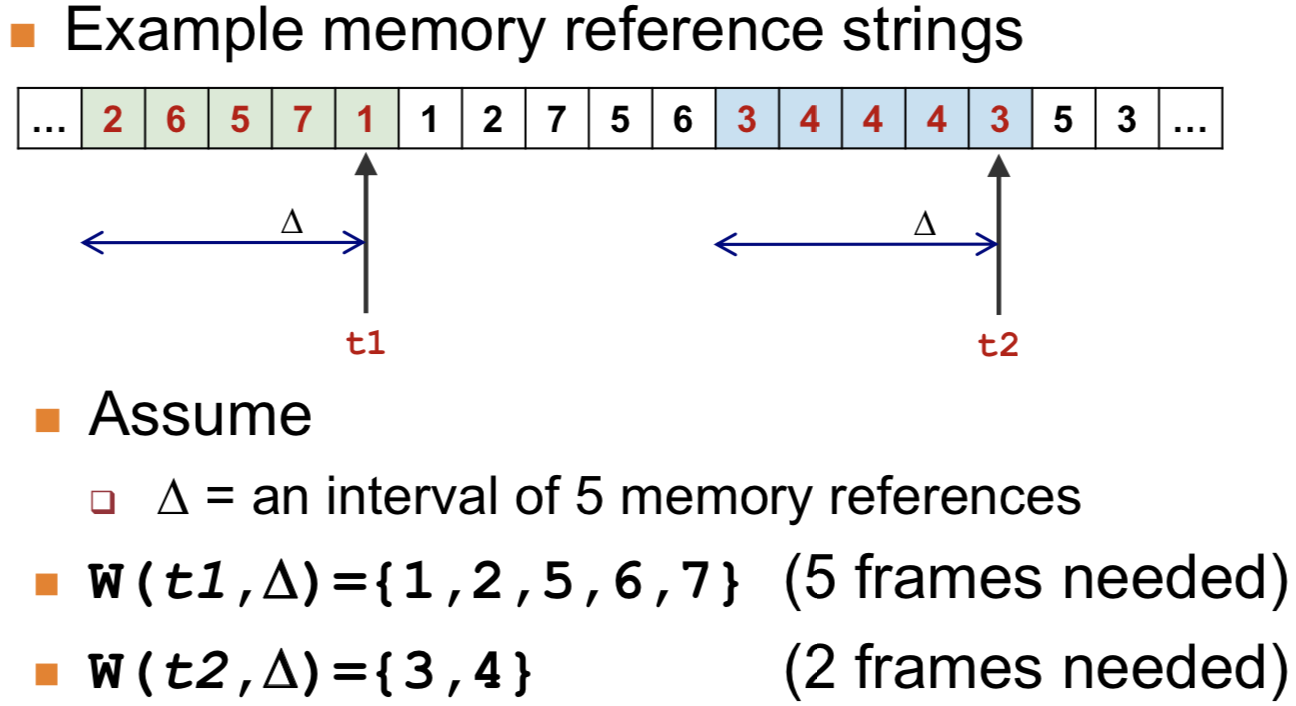
\includegraphics[width=0.75\linewidth]{images/working-set-example}\\
$\Delta$: too small -> miss page in current locality, too big : contains page from different locality.